\section{MARCO TECNOLÓGICO}

El problema que se busca solucionar en este trabajo tiene relación directa con el campo de estudio de la visión por ordenador. Este campo de la Ingeniería Informática busca, 
a través de sistemas de captación y procesamiento de imágenes, generar información y automatizar procesos con ordenadores. \newline Dentro de este campo se han desarrollado tecnologías que usamos día a día
\cite{szeliskiComputerVisionAlgorithms2022}:

\begin{itemize}
    \item \textbf{\textit{\acrfullr{ocr}}} para realizar reconocimiento de texto en imágenes y documentos.
    \item \textbf{Detección de fallos en maquinaria} en procesos de fabricación.
    \item \textbf{Fotogrametría} para mapear imágenes a modelos 3D.
    \item \textbf{Imagen médica} para uso en operaciones a tiempo real\cite{NEMESIS3DCM}.
    \item \textbf{Detección de objetos} en imágenes o videos.
    \item \textbf{Detección de movimiento} y seguimiento de objetos en escenas.
\end{itemize}

Las aplicaciones que usan herramientas basadas en este tipo de soluciones suelen seguir una estructura similar a la siguiente:

\begin{enumerate}
    \item Capturar información a través de cámaras o flujos de video IP de diferentes características.
    \item (A veces) Realizar un preprocesamiento de las imágenes para adaptarlas al sistema.
    \item Procesar las imágenes para extraer información relevante para el sistema.
    \item Transformar la información extraída a través de algoritmos inteligentes para construir una base de datos que sea útil para el usuario de la aplicación.
\end{enumerate}

En el caso de este trabajo, se tratan problemas de detección de objetos y análisis de cambio. Este tipo de tareas se han llevado a cabo antiguamente a través de algoritmos complejos y deterministas, pero en los últimos 
años, con el auge del aprendizaje automático, se ha creado un nuevo paradigma.

En los siguientes puntos se va a describir de forma breve las técnicas de aprendizaje automático, los sistemas de detección de objetos, seguimiento de cambio y los entornos de desarrollo y despliegue 
de estas técnicas de forma transparente al \textit{Hardware} disponible así como proyectos relacionados con este trabajo.
\clearpage

\subsection{Aprendizaje Automático y \textit{Deep Learning}}

\subsubsection{Definición y tipos de tareas}

El campo del aprendizaje automático busca desarrollar soluciones a través de algoritmos y sistemas que permitan a los ordenadores tratar los datos entrantes como el cerebro humano, siendo capaz de 
generalizar las propiedades que les definen y encontrar patrones.

Este aprendizaje automático se realiza sobre un conjunto de datos que aporta el usuario con el objetivo de abstraer diferentes informaciones específicas o agrupar los datos según patrones. Este aprendizaje 
habitualmente se realiza a través de un bucle de tres fases (ver \autoref{fig:FasesAprendizaje}) en las cuales se configura el sistema para aprender, se válida el sistema resultante y se reconfiguran los parámetros para acercarse a un sistema 
que aporte mejores resultados.

\begin{figure}[H]
    \centering
    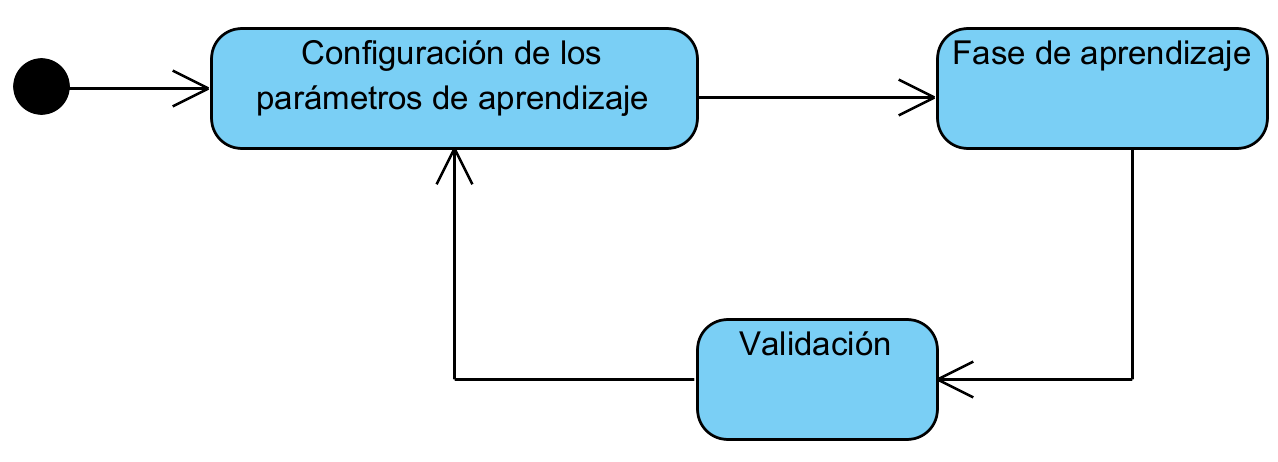
\includegraphics[width=0.7\textwidth]{images/4/Fases.png}
    \caption{Bucle de fases de aprendizaje en un sistema de \textit{Machine Learning}}
    \label{fig:FasesAprendizaje}
\end{figure}

Dentro del campo existen diferentes ramas dependientes del objetivo del aprendizaje que se busca y los datos con los que vamos a alimentar el sistema:

\begin{itemize}
    \item \textbf{Entrenamiento supervisado}: es un tipo de entrenamiento en el que se conoce la relación entre los datos de entrada y los datos esperados. 
    \item \textbf{Entrenamiento no supervisado}: el objetivo de este aprendizaje es aprender las relaciones de los datos de entrada entre sí.
    \item \textbf{Entrenamiento reforzado}: es una variación del entrenamiento supervisado en el que el investigador proporciona feedback sobre los resultados como parte de la fase de aprendizaje. Se utiliza 
    mucho en el ámbito de la robótica.
\end{itemize}

Entre todas las técnicas que implementan este tipo de tareas, uno de los sistemas modernos más conocidos son las redes neuronales.

\subsubsection{Redes Neuronales}

Este campo tiene su origen en una publicación de Warren McCulloch y Walter Pitts en 1943\cite{mccullochLOGICALCALCULUSIDEAS} en el que presentaban la idea de neurona como una unidad lógica básica 
implementable cuyo estado se puede definir como un "todo o nada", lo cual se representa en el campo de las telecomunicaciones con una función escalón como se ve en la \autoref{fig:Escalon}. Este 
trabajo y diseño de neurona sería conocido más tarde como perceptron.

\begin{figure}[H]
    \centering
    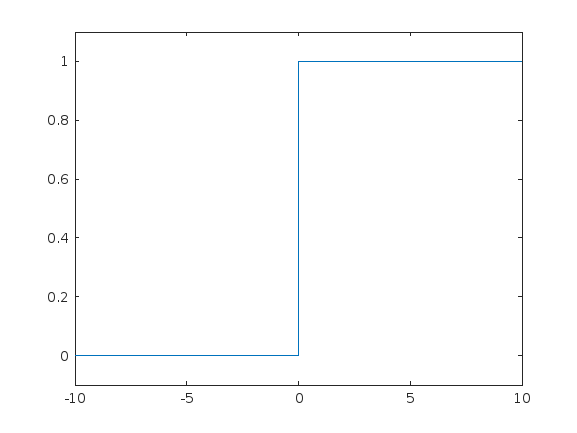
\includegraphics[width=0.3\textwidth]{images/4/Escalon.png}
    \caption{Figura de activación escalón de las primeras neuronas}
    \label{fig:Escalon}
\end{figure}

La estructura básica del perceptron se puede observar en la \autoref{fig:Perceptron} consiste en un nodo con un número \(\mathcal{N}\) de conexiones entrantes, con un peso asociado \(\mathcal{W}\) 
a cada entrada. El nodo calcula el sumatorio de cada conexión con su respectivo peso. Al resultado de este cálculo se le añade un factor de \textit{bias} y por último, mediante una función de 
activación como la vista anteriormente, se decide el resultado de salida de la neurona. 

\begin{figure}[H]
    \centering
    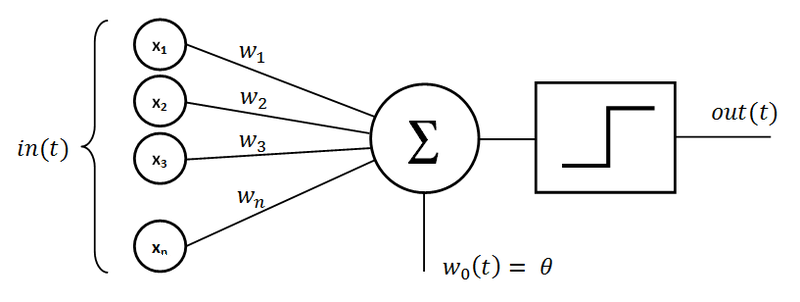
\includegraphics[width=0.5\textwidth]{images/4/perceptron.png}
    \caption{Diagrama general de un perceptron\cite{JgfisherPerceptronPerceptron}}
    \label{fig:Perceptron}
\end{figure}

Más tarde, se conseguiría implementar un diseño electrónico de esta neurona, e interconectar más neuronas entre sí. Estas interconexiones dan lugar a la creación del concepto de \textbf{redes neuronales}, 
siendo una de las primeras redes complejas funcionales de tipo \acrfullr{mlp}. Estos sistemas serían clave para la evolución del aprendizaje automático, apareciendo multitud de 
variaciones en la arquitectura de la red según las necesidades (ver \autoref{fig:ArquitecturasRedes}).

\begin{figure}[H]
    \centering
    \begin{subfigure}[b]{0.25\textwidth}
        \centering
        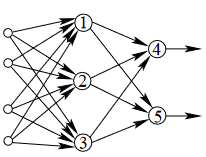
\includegraphics[width=0.9\textwidth]{images/4/FeedForward.png}
        \caption{Red FeedForward}
        \label{fig:a}
    \end{subfigure}
    \begin{subfigure}[b]{0.25\textwidth}
        \centering
        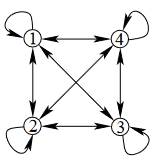
\includegraphics[width=0.7\textwidth]{images/4/Recursiva.png}
        \caption{Red recursiva}
        \label{fig:b}
    \end{subfigure}
    \begin{subfigure}[b]{0.45\textwidth}
        \centering
        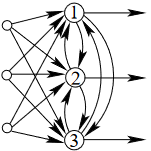
\includegraphics[width=0.4\textwidth]{images/4/FeedForwardLateral.png}
        \caption{Red FeedForward con inhibidores laterales}
        \label{fig:c}
    \end{subfigure}
    \caption{Diferentes ejemplos de arquitecturas simples de redes neuronales\cite{duNeuralNetworksStatistical2013}}
    \label{fig:ArquitecturasRedes}
\end{figure}

El avance progresivo de la capacidad de cómputo de los ordenadores ha permitido el uso de redes neuronales de mayor tamaño, que permiten mayor capacidad de abstracción. Es en este marco donde aparece el término 
\textit{Deep Learning}, que no indica nada más que el uso de redes neuronales con una cantidad masiva de capas intermedias. Además, son sistemas que trabajan muy bien en sistemas con gran grado de paralelización, 
aunque esto se explicará más adelante.

Este tipo de sistemas han demostrado su gran capacidad de abstracción y rapidez, es por esto mismo que las redes neuronales profundas son una de las principales herramientas que se utilizan hoy en día en 
visión por ordenador.

\clearpage
\subsection{Detección de Objetos con redes neuronales}

La detección de objetos como tarea surge de la necesidad de analizar la existencia de objetos en imágenes y; opcionalmente, posicionarlos en las mismas.Para realizar este tipo de tareas se han ido 
desarrollando técnicas tradicionales basadas en algoritmos extremadamente deterministas, pero, con el auge del aprendizaje automático, a partir de 2012\cite{zouObjectDetection202023} 
el paradigma pasó a centrarse en la creación de sistemas detectores basados en \textit{Deep Learning} (Sistemas de Redes Neuronales con una gran cantidad de capas ocultas).

Ambas técnicas se basan en la extracción y el análisis de características de las imágenes, esto es, la caracterización de imágenes o zonas de interés a través de algoritmos o filtros. Podemos entender la caracterización 
de una imagen como la parametrización de los elementos que la definen. Dentro de la vista humana existen muchos elementos que se pueden usar para definir una imagen, algunos ejemplos son:
\begin{itemize}
    \item \textbf{Nitidez}.
    \item \textbf{Color}.
    \item \textbf{Presencia de ciertas formas geométricas}.
    \item \textbf{Brillo}.
    \item \textbf{Ruido}
\end{itemize}

Pero estos ejemplos son características que da un humano para una imagen, las redes neuronales trabajan con características de bajo nivel (P.Ej.: existencia de bordes en una zona específica, colores en un area, 
patrones de puntos, etc.) que permitan analizar zonas de la imagen. Sin embargo, las redes neuronales tipo \textit{\acrshort{mlp}} no están pensadas para obtener características (el análisis de características 
no escala bien con el aumento de resolución), ya que utilizan los valores para realizar la aproximación.

Por estos motivos, se buscó una forma de añadir independencia espacial a la entrada de las redes neuronales. Esto se consigue mediante el uso de diferentes arquitecturas, siendo la más importante las redes 
neuronales convolucionales.\newline

\subsubsection{Redes convolucionales \textit{(CNN)}}

Definen una arquitectura basada en dos pasos: la extracción de las características de las imágenes y la clasificación de las imágenes según las características. Su estructura básica se compone de dos subredes 
que cumplen las dos funciones diferentes para los datos de entrada (ver \autoref{fig:ArquitecturaCNN}).

\begin{figure}[H]
    \centering
    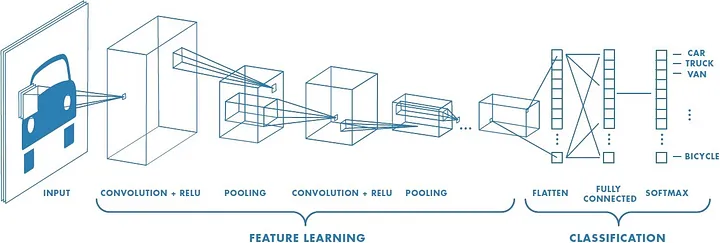
\includegraphics[width=0.9\textwidth]{images/4/ArquitecturaCNN.png}
    \caption{Arquitectura básica de una CNN\cite{sahaComprehensiveGuideConvolutional2022}}
    \label{fig:ArquitecturaCNN}
\end{figure}

\clearpage

La fase de caracterización se compone principalmente de capas neuronales convolucionales y, habitualmente capas de polling:

\begin{itemize}
    \item Capas convolucionales: tienen como objetivo la extracción de carácteristicas a través de neuronas que implementan operaciones de convolución sobre las imágenes. 
    Al ser las imágenes tensores, se les aplican filtros convolucionales implementados a través de \textit{Kernels}. 
    Dependiendo de la característica a buscar, existen diferentes filtros convolucionales y en las fases de entrenamiento se va conformando el \textit{Kernel} que caracteriza mejor esa zona de la imagen para los datos esperados.

    Un ejemplo de \textit{Kernel} es un filtro laplaciano gaussiano como el de la \autoref{fig:LaplaceKernel}, que, a través del gradiente, sirve para darle más énfasis a los bordes de la imagen, como se puede ver 
    en la \autoref{fig:LaplaceResultado}
    \begin{figure}[H]
        \centering
        \(
        \begin{vmatrix}
            1 & 1 & 1 \\
            1 & 8 & 1 \\
            1 & 1 & 1
        \end{vmatrix}
        \)
        \caption{Aspecto de un \textit{kernel} de laplace de tamaño \texttt{3x3}}
        \label{fig:LaplaceKernel}
    \end{figure}
    \begin{figure}[H]
        \centering
        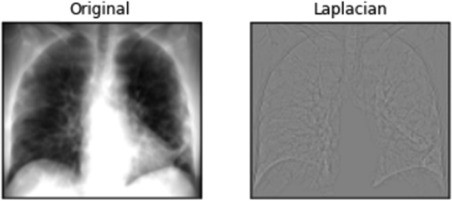
\includegraphics[width=0.5\textwidth]{images/4/KernelsTipicos.jpg}
        \caption{Aplicación de un filtro gaussiano de Laplace a una imagen médica\cite{LaplacianFilterOverview}}
        \label{fig:LaplaceResultado}
    \end{figure}

    Estas capas convolucionales van obteniendo la abstracción de las características transformando los volúmenes de entrada a volúmenes de salida de mayor profundidad pero de menor resolución vertical y horizontal.

    \item Capas de polling: Su objetivo es ir haciendo sub-muestreo de las capas convolucionales superiores para conformar el volumen de entrada de la siguiente capa convolucional, reduciendo la carga computacional necesaria. 
    Se puede ver su funcionamiento en la \autoref{fig:MuestreoCNN}, donde sub-muestrean un volumen de resolución \texttt{28x28} a una resolución \texttt{14x14}.
    \begin{figure}[H]
        \centering
        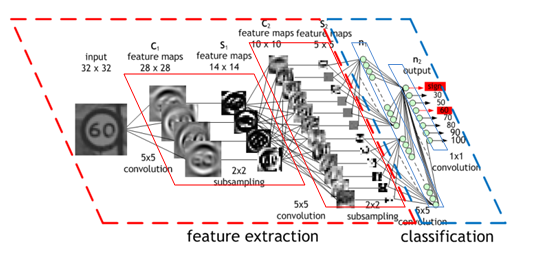
\includegraphics[width=0.6\textwidth]{images/4/EjemploPolling.png}
        \caption{CNN con detalle de la caracterización y el sub-muestreo\cite{ConvolutionalNeuralNetwork}}
        \label{fig:MuestreoCNN}
    \end{figure}

\end{itemize}

La fase de clasificación habitualmente usa una red neuronal profunda conectada completamente entre capas como se ha podido ver en la anterior sección, similar a la idea de una \textit{\acrshort{mlp}}. Esta 
red toma como entrada un vector aplanado final de la parte de extracción de características y realiza la clasificación.

\subsubsection{Redes neuronales para acuicultura}

El uso de una red neuronal para solucionar un problema está asociado al tipo de trabajo a realizar. Cuando se define un problema en el que se va a aplicar esta técnica, normalmente cae en tres tipos de 
categorías(ver \autoref{fig:tareasCNN}). Además, esta selección tiene unas implicaciones en la complejidad computacional de la tarea, ya que la capa de clasificación debe ser cambiada para soportarla.

\begin{itemize}
    \item Clasificación: las imágenes son marcadas dependiendo de si existe (binario) un elemento dentro de ella.
    \item Detección de objetos: regiones locales de la imagen son clasificadas y marcadas dependiendo de la existencia del elemento en cuestión.
    \item Segmentación semántica: se realiza una clasificación por cada pixel para delimitar todos los píxeles que conforman la instancia del objeto
\end{itemize}

\begin{figure}[H]
    \centering
    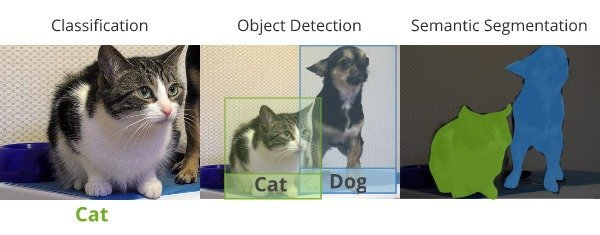
\includegraphics[width=0.6\textwidth]{images/4/TiposTareas.png}
    \caption{Tareas típicas de una CNN\cite{kallfelzsirmacekSEQUENTIALIMAGEPROCESSING2019}}
    \label{fig:tareasCNN}
\end{figure}

La evolución de las \textit{\acrshort{cnn}} ha sido exponencial y han aparecido arquitecturas que han ido añadiendo mejoras de eficiencia, calidad de resultados y estándares a la hora de crear nuevos 
sistemas:
\begin{itemize}
    \item R-CNN (Region-CNN)(2014): introdujo el análisis solo en regiones con datos interesantes.
    \item Fast R-CNN (2015): mejora R-CNN introduciendo búsqueda selectiva, definiendo un número máximo de \acrfullr{roi} a tratar.
    \item Faster R-CNN (2015).
    \item YOLO (You Only Look Once)\cite{redmonYouOnlyLook2016}: arquitectura extremadamente rápida perteneciente al estado del arte moderno en redes neuronales, que ha ido mejorandose en forma de versiones.
\end{itemize}

Cada arquitectura ha traído consigo mejoras y a veces, a cambio de perdida de rendimiento. Esto es un problema que debe tenerse en cuenta y existen diversos trabajos\cite{hanAdvancedDeepLearningTechniques2018}\cite{manojkumarPerformanceComparisonReal2023}\cite{bhagyaOverviewDeepLearning2019} 
que tratan simplemente las diferencias existentes entre diferentes arquitecturas.\newline
Uno de estos trabajos\cite{hanAdvancedDeepLearningTechniques2018} compara diferentes arquitecturas contra el conjunto de datos de la universidad de Oxford "Pascal2012"\cite{PASCALVisualObject}, que contiene 20 clases de objetos.\newline
Como resultado de este análisis; resumido en la \autoref{ResumenCNN}, se puede observar que YOLOv2, aún no siendo el mejor, tiene un rendimiento bastante competente. Si nos quedásemos con solo este dato, podriamos pensar que YOLO 
no tiene porque ser la mejor elección, pero hay que tener en cuenta el factor de rendimiento, que se mide principalmente en el tiempo que se tarda en realizar la inferencia en una imagen. En este caso, podemos observar 
que YOLOv2 es capaz de superar a SSD512 obteniendo un mejor \acrfullr{map}(parámetro de caracterización del error medio generalizado sobre todo el dataset) con el doble de rendimiento.

\begin{table}[h]
    \begin{center} {\footnotesize
    \begin{tabular}{lcccc}
    \hline
     & \multicolumn{1}{c}{bike} & \multicolumn{1}{c}{bird} & \multicolumn{1}{c}{train} & \multicolumn{1}{c}{mAP}\\
    \hline
    \raisebox{0ex}{Faster R-CNN} & 81.6 & 77.2 & 84.7 & 73.8\\[0ex]
    \raisebox{0ex}{SSD300} & 80.1 & 70.5 & 81.9 & 72.4\\[0ex]
    \raisebox{0ex}{SSD512} & 82.3 & 75.8 & 86.3 & 74.9\\[0ex]
    \raisebox{0ex}{YOLO} & 67.2 & 57.7 & 73.9 & 57.9\\[0ex]
    \raisebox{0ex}{YOLOv2 $544x544$} & 82.0 & 74.8 & 83.8 & 73.4\\[0ex]
    \hline
    \end{tabular} }
    \end{center}
    \caption{\footnotesize Resumen de la comparación entre CNN con el dataset PASCAL2012\cite{hanAdvancedDeepLearningTechniques2018}}
    \label{ResumenCNN}
\end{table}

\begin{table}[h]
    \begin{center} {\footnotesize
    \begin{tabular}{lcc}
    \hline
     & \multicolumn{1}{c}{mAP} & \multicolumn{1}{c}{FPS}\\
    \hline
    \raisebox{0ex}{Faster R-CNN} & 76.4 & 5\\[0ex]
    \raisebox{0ex}{SSD300} & 74.3 & 46\\[0ex]
    \raisebox{0ex}{SSD512} & 76.8 & 19\\[0ex]
    \raisebox{0ex}{YOLO} & 63.4 & 45\\[0ex]
    \raisebox{0ex}{YOLOv2 $544x544$} & 78.6 & 40\\[0ex]
    \hline
    \end{tabular} }
    \end{center}
    \caption{\footnotesize Detalle de rendimiento en \acrshort{fps} en la comparativa\cite{hanAdvancedDeepLearningTechniques2018}}
    \label{ResumenCNNFPS}
\end{table}

Estos resultados comparativos, a diferencias de otros artículos, sirven como marco por el uso de reglas tales como la comparación bajo mismo dataset e indicar tamaño de imagen de entrada a la red neuronal.




\subsection{Técnicas para el análisis  de movimiento en la visión por ordenador}

\subsubsection{Definición y uso del análisis de flujo óptico}

\subsubsection{Uso en acuicultura}

\subsubsection{Problemas asociados}

\subsection{Entornos de desarrollo, sistemas de despliegue y \textit{Hardware} transparente}